\section{Results}
\subsection{Effect of Value Selection on ASR}
Tables~\ref{tab:ember2018_1p_if} and \ref{tab:ember2024_1p_if} report a representative run at a 1\% poison rate using Isolation Forest as a compact detectability baseline.
Additional runs with several random seeds, higher poison rates, and other sanitizer baselines were used to check whether the same qualitative pattern appeared.
The main text focuses on the 1\% Isolation Forest setting because it compactly shows how value selection changes ASR and poison recall.

The results indicate that trigger value selection strongly affects attack success even when the trigger feature set is fixed.
The Severi-derived selectors, especially MinPopulation and CountAbsSHAP, achieve very high ASR under distribution-based distance sampling on both datasets.
On EMBER 2018, they achieve 98.35\% and 98.73\% ASR, respectively, while on EMBER 2024 Win64 they achieve 99.09\% and 99.04\%.
This confirms that rare-value and low-SHAP-contribution value selection can produce effective triggers.

Among the extended selectors, CorrCountAbsSHAP also maintains high ASR under distribution-based sampling, reaching 92.72\% on EMBER 2018 and 98.43\% on EMBER 2024 Win64.
Q95 achieves 94.99\% ASR on EMBER 2018 and 88.65\% on EMBER 2024 Win64. By contrast, CombinedSHAP and BenignPrototype generally achieve lower ASR, particularly under random sampling.
Overall, the results indicate that the selected trigger values substantially change attack effectiveness, even when the trigger features and poisoning protocol are held constant.

\begin{table}[!t]
    \centering
    \caption{EMBER 2018 results at a 1\% poison rate using Isolation Forest.}
    \label{tab:ember2018_1p_if}
    \setlength{\tabcolsep}{2.0pt}
    \renewcommand{\arraystretch}{1.08}
    \begin{tabular}{llrrrr}
        \toprule
        \textbf{Sampling} &
        \textbf{Selector} &
        \textbf{ASR} &
        \makecell{\textbf{Poison}\\\textbf{Recall}} &
        \makecell{\textbf{Poisons}\\\textbf{Removed}} &
        \makecell{\textbf{Benign}\\\textbf{Removed}} \\
        \midrule
        Random & MinPopulation*      & 87.98 & 100.00 & 1200 &    0 \\
               & CountAbsSHAP*    & 74.16 & 100.00 & 1200 &    0 \\
               & CombinedSHAP*     & 52.55 &   0.17 &    2 & 1198 \\
               & FreqBoundedSigned    & 54.81 &  91.00 & 1092 &  108 \\
               & LowSignedSHAP       & 83.65 &  97.83 & 1174 &   26 \\
               & CorrCountAbsSHAP  & 36.41 &   5.25 &   63 & 1137 \\
               & BenignPrototype   &  4.65 &   0.08 &    1 & 1199 \\
               & Q95           & 39.32 &  21.58 &  259 &  941 \\
        \midrule
        Distribution-based
               & MinPopulation*      & 98.35 & 100.00 & 1200 &    0 \\
               & CountAbsSHAP*    & 98.73 &  99.42 & 1193 &    7 \\
               & CombinedSHAP*     & 87.61 &   0.00 &    0 & 1200 \\
               & FreqBoundedSigned    & 93.57 &  85.58 & 1027 &  173 \\
               & LowSignedSHAP       & 88.79 &  97.25 & 1167 &   33 \\
               & CorrCountAbsSHAP  & 92.72 &   1.92 &   23 & 1177 \\
               & BenignPrototype   & 29.99 &   0.00 &    0 & 1198 \\
               & Q95           & 94.99 &   2.75 &   33 & 1167 \\
        \bottomrule
    \end{tabular}
    \vspace{0.5mm}
    \raggedright
    * indicates selectors derived from Severi et al.
\end{table}
\begin{table}[!t]
    \centering
    \caption{EMBER 2024 Win64 results at a 1\% poison rate using Isolation Forest.}
    \label{tab:ember2024_1p_if}
    \setlength{\tabcolsep}{2.0pt}
    \renewcommand{\arraystretch}{1.08}
    \begin{tabular}{llrrrr}
        \toprule
        \textbf{Sampling} &
        \textbf{Selector} &
        \textbf{ASR} &
        \makecell{\textbf{Poison}\\\textbf{Recall}} &
        \makecell{\textbf{Poisons}\\\textbf{Removed}} &
        \makecell{\textbf{Benign}\\\textbf{Removed}} \\
        \midrule
        Random & MinPopulation*      & 17.12 & 100.00 & 2080 &    0 \\
               & CountAbsSHAP*    & 15.20 & 100.00 & 2080 &    0 \\
               & CombinedSHAP*     &  6.84 &   1.73 &   36 & 2044 \\
               & FreqBoundedSigned    & 15.71 &  79.23 & 1648 &  432 \\
               & LowSignedSHAP       & 19.73 &  99.33 & 2066 &   12 \\
               & CorrCountAbsSHAP  & 11.93 &   4.33 &   90 & 1990 \\
               & BenignPrototype   &  2.63 &   0.00 &    0 & 2078 \\
               & Q95           & 10.96 &  16.44 &  342 & 1738 \\
        \midrule
        Distribution-based
               & MinPopulation*      & 99.09 & 100.00 & 2080 &    0 \\
               & CountAbsSHAP*    & 99.04 & 100.00 & 2080 &    0 \\
               & CombinedSHAP*     & 59.96 &   2.88 &   60 & 2020 \\
               & FreqBoundedSigned    & 95.80 &  65.77 & 1368 &  710 \\
               & LowSignedSHAP       & 93.29 &  98.13 & 2041 &   36 \\
               & CorrCountAbsSHAP  & 98.43 &  12.55 &  261 & 1819 \\
               & BenignPrototype   & 53.10 &   0.00 &    0 & 2080 \\
               & Q95           & 88.65 &  27.84 &  579 & 1501 \\
        \bottomrule
    \end{tabular}
    \vspace{0.5mm}
    \raggedright
    * indicates selectors derived from Severi et al.
\end{table}

\subsection{Detectability Profiles}
Fig.~\ref{fig:asr-defense-profile} visualizes the effectiveness--detectability profile by plotting ASR against Isolation Forest poison recall.
Points in the upper-right region are effective but easy to detect, whereas points in the upper-left region are effective and harder to detect.

\begin{figure}[!t]
    \centering
    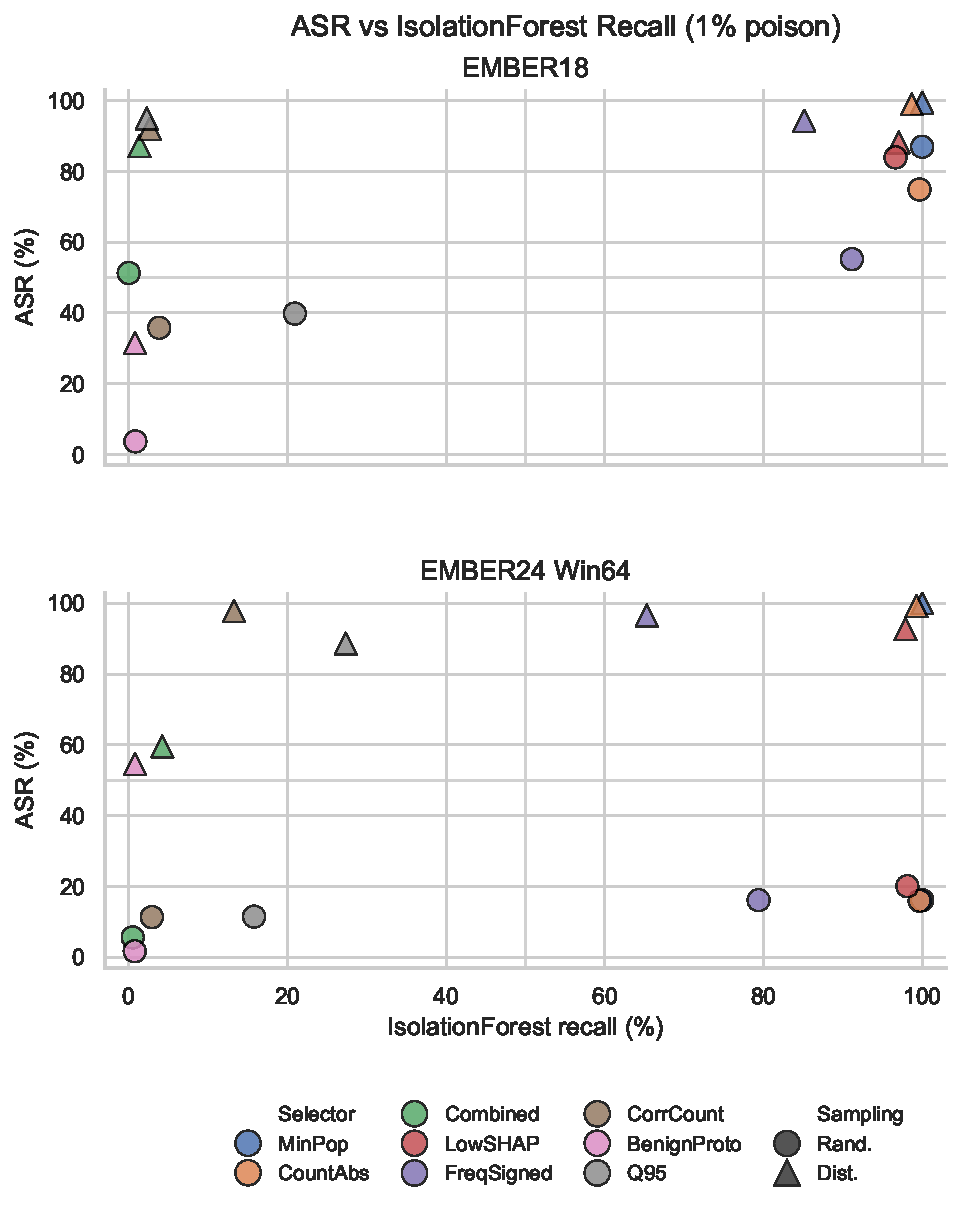
\includegraphics[width=\columnwidth]{figure/asr_vs_isolation_forest_recall_1p.pdf}
    \caption{Attack effectiveness versus Isolation Forest detectability at 1\% poison rate. ASR/evasion is plotted against poison recall for EMBER 2018 and EMBER 2024 Win64.}
    \label{fig:asr-defense-profile}
\end{figure}

As shown in Tables~\ref{tab:ember2018_1p_if} and~\ref{tab:ember2024_1p_if}, MinPopulation and CountAbsSHAP occupy the high-ASR and high-recall region under distribution-based distance sampling.
Under random sampling, they remain highly exposed to Isolation Forest, but their ASR can be much lower, especially on EMBER 2024 Win64.
In contrast, CombinedSHAP, CorrCountAbsSHAP, BenignPrototype, and Q95 achieve lower poison recall but differ in how much ASR they preserve.
CombinedSHAP and BenignPrototype can reduce poison recall, but this reduction often comes with substantial ASR loss.
CorrCountAbsSHAP is more attractive because it preserves high ASR under distribution-based distance sampling while keeping poison recall much lower than the strongest Severi-derived baselines.
FrequencyBoundedSignedSHAP shows an intermediate profile, retaining relatively high ASR under distribution-based sampling while remaining moderately exposed to sanitization.
LowSignedSHAP is closer to the aggressive selectors, achieving high ASR but also very high poison recall on both datasets.

Compared with CountAbsSHAP, CorrCountAbsSHAP reduces poison recall from 99.42\% to 1.92\% on EMBER 2018 and from 100.00\% to 12.55\% on EMBER 2024 Win64 under distribution-based sampling, while retaining ASR of 92.72\% and 98.43\%, respectively.
Q95 shows a favorable effectiveness–detectability profile.
It achieves 94.99\% ASR with 2.75\% poison recall on EMBER 2018 and 88.65\% ASR with 27.84\% poison recall on EMBER 2024 Win64. In comparison, MinPopulation and CountAbsSHAP achieve approximately 98–99\% ASR but approximately 99–100\% poison recall.

We also evaluated HDBSCAN and Spectral Signature to check whether the observations are specific to Isolation Forest.
Although the exact poison recall varies across sanitizers, the additional results support the same general pattern: aggressive selectors such as MinPopulation, CountAbsSHAP, and LowSignedSHAP are often more exposed to sanitization, whereas CorrCountAbsSHAP and Q95 show more favorable effectiveness–detectability profiles.
Evaluating ASR alone can therefore be misleading, because a highly effective attack may still be neutralized if most poisoned samples are removed before retraining.

\subsection{Effect of Sampling Strategy}
Sampling strategy also has a strong effect on attack effectiveness.
Distribution-based distance sampling consistently improves ASR compared with random sampling, especially on EMBER 2024 Win64.
This is consistent with PMSB-style sampling, where poisoning malware-similar benign samples makes the trigger easier for the model to associate with the benign class because these samples are closer to the decision boundary.

However, sampling strategy does not remove the role of value selection.
Even under distribution-based distance sampling, selectors still differ substantially in both ASR and poison recall.
This means that sample selection and value selection control different parts of the attack.
PMSB-style sampling determines which benign samples are poisoned, whereas value selection determines which trigger pattern is learned from those poisoned samples.
Thus, PMSB-style sampling can strengthen the attack, but the resulting effectiveness–detectability profile still depends on the selected trigger values.